This section discusses the results for minimax Q-learning. Due to time constraints, this part of the assignment was only executed on a 5.5 grid. The behaviour of this algorithm has lead to running 100 episodes over 20 experiments in order to generate results. Also, the default values were changed in order to get minimax-Q to work. These default values are a learning rate of 0.5, a discount factor of 0.2 and an epsilon value of 

\subsection{1 predator versus 1 prey}
This section discusses the results of 
\begin{center}
	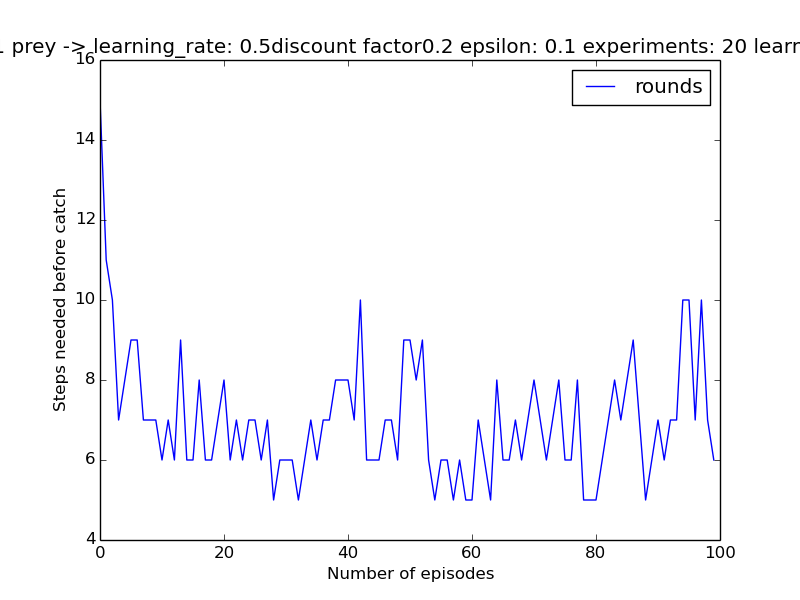
\includegraphics[scale=0.3]{minimax_100rounds_20exp_disc02_alpha05}
	\captionof{figure}{Minimax-Q: 1 predator versus 1 prey, with discount factor of 0.2}
	\label{graph:1vs1_disc_02}
\end{center}

\begin{center}
	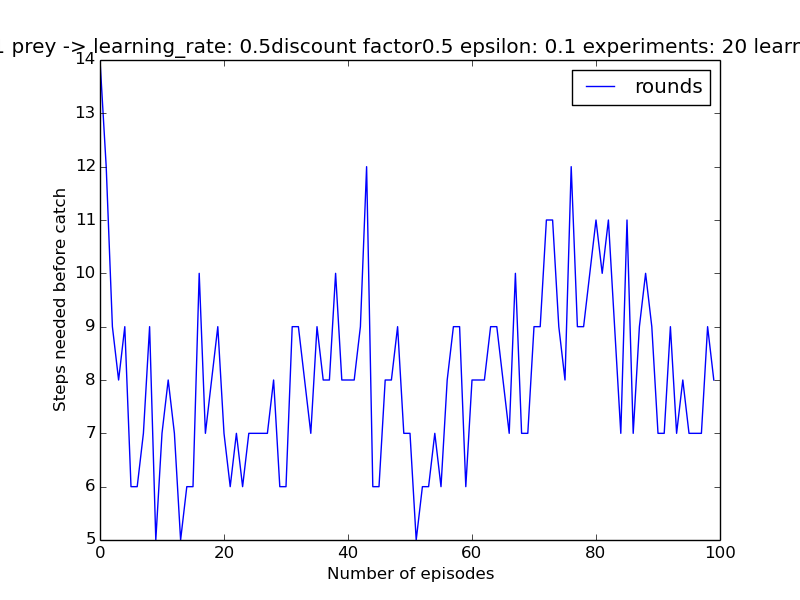
\includegraphics[scale=0.3]{minimax_100rounds_20exp_disc05_alpha05}
	\captionof{figure}{Minimax-Q: 1 predator versus 1 prey, with discount factor of 0.5}
	\label{graph:1vs1_disc_05}
\end{center}

\begin{center}
	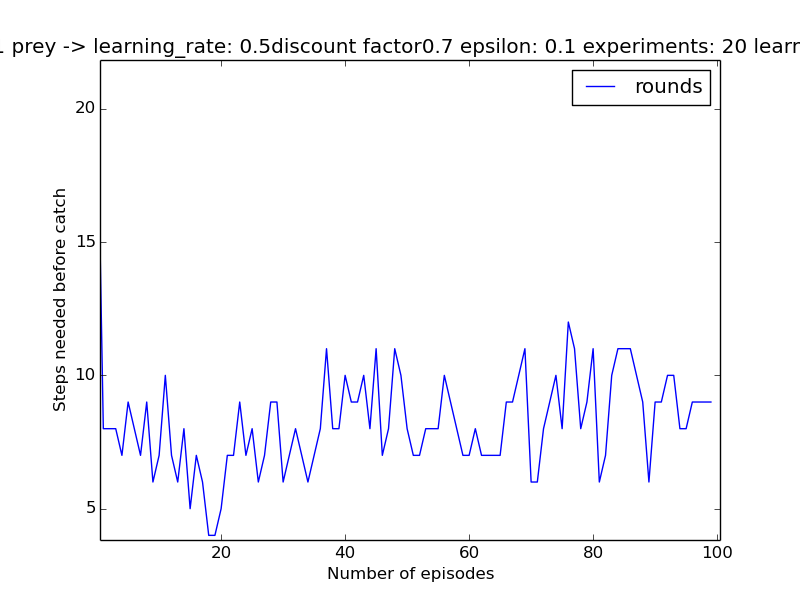
\includegraphics[scale=0.3]{minimax_100rounds_20exp_disc07_alpha05}
	\captionof{figure}{Minimax-Q: 1 predator versus 1 prey, with discount factor of 0.7}
	\label{graph:1vs1_disc_07}
\end{center}

Thought the results seem very noisy, it is clear that a low discount factor yields best results. Again, this is essential to ensure that the predators do not collide.